% \makeatletter \def\NR@nopatch@beamer{} \makeatother
\documentclass[xcolor=dvipsnames, onlymath, 10pt, aspectratio=169, handout]{beamer}
\usecolortheme[named=Black]{structure}
% \usepackage{etex} % Too many packages

\usepackage[utf8]{inputenc}
\usepackage[T1]{fontenc}
\usepackage{tipa}
\usepackage{color}
\usepackage{natbib}

\usepackage[french,english]{babel}
\usepackage{multicol}
\usepackage{caption}
\usepackage{vowel}
\usepackage{diagbox}
\usepackage{fontawesome}
\usepackage{color}
\usepackage{tikz-qtree}
\usepackage{booktabs}
\usepackage{hyperref}
\usepackage{bibentry}
\usepackage{arydshln}
\usepackage{linguex}
\usetikzlibrary{arrows.meta, shapes, arrows, positioning, calc, trees}
\usepackage{pifont}
\usepackage{textgreek}
% \usepackage{eulervm}
\usepackage{libertinus}
\usepackage{inconsolata}
\usepackage{datetime}

\definecolor{pastelorange}{RGB}{255,179,71}


% ============ >>>> MAC

\input{/Users/gdgarcia/Dropbox/Academia/LaTeX/garcia_latex_commands.tex}


% COURSE:

\newcommand{\course}{LNG-1100 : Méthodes expérimentales\\et analyse de données}

% TOPIC:

\newcommand{\classtopic}{\vspace{2ex}Question de recherche, collecte de données, intro à R}

% DATE:

\newcommand{\classdate}{\fbox{2}}

% =====================================
% =====================================
% =====================================


% Define header colors:
\definecolor{lav1}{RGB}{184, 0, 35}
\definecolor{lav2}{RGB}{246, 195, 67}




\setbeamertemplate{itemize item}{$\bullet$}
\setbeamertemplate{itemize subitem}{$\circ$}
\setbeamerfont{frametitle}{series=\bfseries}
\setbeamercolor{frametitle}{fg=lav,bg=white}
\setbeamerfont{title}{series=\bfseries, parent=structure}
\setbeamercolor{title}{fg=lav,bg=white}



\usepackage[most]{tcolorbox}

    \tcbset{
        enhanced,
        colback=lavb!5!white,
        boxrule=0.1pt,
        colframe=lavb!80!white,
        fonttitle=\bfseries,
        width=5cm, box align=top,
        nobeforeafter
       }

\renewcommand\bibsection{\section[]{\refname}}
\usetheme{boxes}            % Simple and clear
\setbeamercolor{button}{bg=black,fg=white}
\beamertemplatenavigationsymbolsempty  % Remove nav controls




\title{\course}

\subtitle{\classtopic}

\author{Guilherme D.\ Garcia}


\institute[Université Laval] % (optional, but mostly needed)
{
  \mylink{https://fr.gdgarcia.ca}{fr.gdgarcia.ca}\vspace{5ex}
}


\date{\classdate}

\subject{Linguistique}


\begin{document}


\begin{frame}
	\vspace{2ex}
	\textcolor{lav1}{\noindent\rule{0.66\textwidth}{3pt}}
	\textcolor{lav2}{\noindent\rule{0.33\textwidth}{3pt}}

	\titlepage

	\vfill

	\begin{center}
		{\includegraphics[width=2.5cm]{/Users/gdgarcia/Dropbox/Academia/Admin/Uni-logos/ULaval1.png}}
	\end{center}

\end{frame}

\addtobeamertemplate{navigation symbols}{}{%
	\usebeamerfont{footline}%
	\usebeamercolor[fg]{footline}%
	\hspace{1em}%
	\vspace{1ex}%
	{\insertframenumber} sur {\inserttotalframenumber}
}



\setbeamertemplate{background}{\tikz[overlay,remember picture]\node[opacity=0.4, xshift=-1cm, yshift=.8cm] at (current page.south east){\includegraphics[width=.75cm]{/Users/gdgarcia/Dropbox/Academia/Admin/Uni-logos/ULaval2bw.png}};}

% ==================================
%  
%
% 
%    
%\end{frame}

% =======================

% =======================

% =======================

\begin{frame}{Plan de la séance}

	\begin{enumerate}
		\item Question de recherche et collecte de données
		\item Intro à R \citep[chapitres 1--3; 5--7]{barnier_R}
		\item Pratique
	\end{enumerate}

\end{frame}

% ==================



\begin{frame}{Question de recherche}

	\begin{itemize}
		\item[\winner] Vos questions déterminent vos méthodes (collecte + analyse)
		\item[1.] Choisissez un sujet qui vous intéresse
		\item[2.] Développez des questions de recherche
		      \begin{itemize}

			      \pause

			      \item \textbf{Examinez les études déjà publiées} (p.\ ex., vers la fin des articles)

			            \pause
			      \item Discutez avec vos collègues et profs
			            \pause
			      \item Explorez des données existantes et observez les patrons qui émergent
			      \item[]
			            \pause

			      \item[\winner] Votre question ne doit pas être trop spécifique ni trop générale :

		      \end{itemize}
	\end{itemize}


	\vspace{2ex}

	\begin{center}
		\begin{tikzpicture}[scale=0.7]

			% Draw the horizontal line
			\draw[thick, ->] (0,0) -- (10,0);

			% Label the ends
			\node[below] at (0,0) {trop spécifique};
			\node[below] at (10,0) {trop générale};

			% Draw a circle somewhere in between
			\filldraw[color=lav] (5,0) circle (5pt);

		\end{tikzpicture}
	\end{center}

	\pause

	\begin{itemize}
		\item[3.] Considérez des résultats possibles et les étapes suivantes
	\end{itemize}

\end{frame}


% =====================

\begin{frame}[t]{Question de recherche}{Exemples}

	\footnotesize

	\begin{importanttitle}{Ordonnez les questions (spécifique $\rightarrow$ générale)}


		\begin{enumerate}
			\item[A.] Comment les locuteurs du français montréalais produisent-ils les voyelles nasales [\textipa{\~A}] et [\textipa{\~E}]\footnote{Par exemple, \fr{temps} et \fr{pain}.} en langage familier?
			      % Cette question est plus spécifique car elle se concentre sur un ensemble spécifique de phonèmes, dans un dialecte spécifique, dans un contexte de parole particulier.

			\item[B.] Quelle est la variation exacte de la fréquence fondamentale (F0)\footnote{La fréquence initiale d'un son brut généré dans les cordes vocales.} pour la voyelle [\textipa{i}] dans le mot ``si'' lorsqu'elle est prononcée par des locuteurs bilingues français-anglais montréalais?
			      % Cette question est excessivement spécifique car elle réduit la recherche à un tel degré qu'elle ne serait probablement pas généralisable ou largement applicable.

			\item[C.] Qu'est-ce qui influence la langue?
			      % Cette question est excessivement large et ne se concentre sur aucun aspect particulier comme la syntaxe, la sémantique, la phonologie, la sociolinguistique, etc.

			\item[D.] Quel est le rôle des processus phonologiques dans l'harmonie vocalique\footnote{Le processus dans lequel une voyelle devient plus similar à une autre voyelle : l\underline{o}tu $\rightarrow$ l\underline{u}tu.} du finnois?
			      % Cette question réduit la zone d'intérêt aux processus phonologiques et spécifie une langue particulière (le finnois) et un phénomène particulier (l'harmonie vocalique).

			\item[E.] Comment les facteurs sociaux affectent-ils le changement linguistique?
			      % Cette question est toujours assez large mais réduit le focus à l'intersection des facteurs sociaux et du changement linguistique.
		\end{enumerate}
	\end{importanttitle}


\end{frame}


% =====================

\begin{frame}[t]{Question de recherche}{Exemples}


	\begin{importanttitle}{Ordonnez les questions (spécifique $\rightarrow$ générale)}


		\begin{enumerate}

			\item[B.] Quelle est la variation de la fréquence fondamentale (F0) pour la voyelle [\textipa{i}] dans le mot \fr{si} lorsqu'elle est prononcée par des locuteurs bilingues français-anglais montréalais?
			      % Cette question est excessivement spécifique car elle réduit la recherche à un tel degré qu'elle ne serait probablement pas généralisable ou largement applicable.

			\item[A.] Comment les locuteurs du français montréalais produisent-ils les voyelles nasales [\textipa{\~A}] et [\textipa{\~E}] en langage familier?
			      % Cette question est plus spécifique car elle se concentre sur un ensemble spécifique de phonèmes, dans un dialecte spécifique, dans un contexte de parole particulier.


			\item[D.] Quel est le rôle des processus phonologiques dans l'harmonie vocalique du finnois?
			      % Cette question réduit la zone d'intérêt aux processus phonologiques et spécifie une langue particulière (le finnois) et un phénomène particulier (l'harmonie vocalique).

			\item[E.] Comment les facteurs sociaux affectent-ils le changement linguistique?
			      % Cette question est toujours assez large mais réduit le focus à l'intersection des facteurs sociaux et du changement linguistique.

			\item[C.] Qu'est-ce qui influence la langue?
			      % Cette question est excessivement large et ne se concentre sur aucun aspect particulier comme la syntaxe, la sémantique, la phonologie, la sociolinguistique, etc.
		\end{enumerate}
	\end{importanttitle}


\end{frame}

% ====================


% =====================
\begin{frame}{Votre projet de recherche}{}
	\begin{itemize}
		\item Un projet de recherche doit être \lav{réaliste}, cela veut dire que :
		      \begin{enumerate}
			      \item vous avez le \lav{temps} pour suivre toutes les étapes nécessaires
			      \item vous avez la \lav{connaissance de base} exigée dans le projet
			      \item vous connaissez les aspects \lav{techniques} et \lav{logistiques}\footnote{Approbation éthique, collecte de données, paiement des participants, accès aux équipements, etc.} impliqués
		      \end{enumerate}

		\item[\winner] Un projet prend le temps, même si les points 1--3 sont très clairs
		\item[]
		      \pause
		\item \textbf{Deux problèmes typiques :}
		      \begin{itemize}
			      \item on sous-estime le temps et la difficulté des étapes nécessaires
			      \item on est trop générale dans notre question ou dans notre sujet de recherche
		      \end{itemize}
	\end{itemize}
\end{frame}
% =====================


\begin{frame}{Collecte de données}{Logiciels}

	\begin{itemize}
		\item Plusieurs méthodes d'élicitation de données exigent des logiciels spécifiques
		\item Quelques options :
		      \begin{itemize}
			      \item \mylink{http://www.psychopy.org}{PsychoPy}, \mylink{https://osdoc.cogsci.nl}{OpenSesame}, \mylink{http://www.fon.hum.uva.nl/praat/}{Praat} \hfill gratuits
			      \item \mylink{https://www.sr-research.com/experiment-builder/}{Experiment builder}, \mylink{https://pstnet.com/products/e-prime/}{E-prime}, \mylink{https://www.mathworks.com/products/matlab.html}{MatLab}, \mylink{https://cedrus.com/superlab/index.htm}{SuperLab}	\hfill \$\$\$
		      \end{itemize}
		\item En plus, \lav{numbreuses} options pour des expériences en ligne
		\item[]
		\item[\winner] Tout cela dépend de votre \lav{question de recherche}
	\end{itemize}

\end{frame}



% ================

\begin{frame}{Bases de données}

	\begin{itemize}
		\item[] De quel type de données avez-vous besoin...?
		\item Écrites? Facile à collecter, mais parfois difficile à analyser
		\item Orales? Comment coder les données?
		\item Jugement?
		\item etc.
	\end{itemize}

\end{frame}



% ================

\begin{frame}{Bases de données}{OSF}

	\begin{itemize}
		\item Base de **données** générale (plusieurs domaines/sujets) : \mylink{https://osf.io}{osf.io}
		\item L'option la plus importante actuellement
		\item *preprints* + matériels supplémentaires (y compris des données, des *scripts*, etc.)

	\end{itemize}

	\begin{center}
		{
\includegraphics[width = 0.5\textwidth]{osf}}
	\end{center}

\end{frame}


% =================


% ================

\begin{frame}{Bases de données}{IRIS}

	\begin{itemize}
		\item Base de données des études sur une langue seconde : \mylink{https://www.iris-database.org}{iris-database.org}
	\end{itemize}

	\begin{center}
		\fbox{\includegraphics[width = 0.5\textwidth]{iris}}
	\end{center}

\end{frame}


% =================


\begin{frame}{Bases de données}{CHILDES}

	\begin{itemize}
		\item[] Spécifique pour l'acquisition du langage\footnote{Une partie du projet \myLink{https://talkbank.org}{TalkBank}.} : \mylink{https://childes.talkbank.org}{childes.talkbank.org}
		\item[]
	\end{itemize}

	\begin{center}
		\fbox{\includegraphics[width = 0.5\textwidth]{childes}}
	\end{center}


\end{frame}


% ==================


\begin{frame}{Bases de données}{WALS}

	\begin{itemize}
		\item[] Excellente base de données sur des traits linguistiques : \mylink{https://wals.info}{wals.info}
		\item[]
	\end{itemize}

	\begin{center}
		\fbox{\includegraphics[width = 0.4\textwidth]{wals}}
	\end{center}


\end{frame}


% ==================


\begin{frame}{Bases de données}{Speech accent archive}

	\begin{itemize}
		\item[] Les accents natifs ou non natifs de l'anglais : \mylink{http://accent.gmu.edu}{accent.gmu.edu}
	\end{itemize}

	\begin{center}
		\fbox{\includegraphics[width = 0.5\textwidth]{accent}}
	\end{center}


\end{frame}

% ==================

\begin{frame}{Bases de données}{CMU Pronouncing Dictionary}

	\begin{itemize}
		\item \mylink{http://www.speech.cs.cmu.edu/cgi-bin/cmudict}{speech.cs.cmu.edu/cgi-bin/cmudict}
	\end{itemize}

	\begin{center}
		\fbox{\includegraphics[width = 0.4\textwidth]{cmu}}
	\end{center}


\end{frame}


% ==================

\begin{frame}{Bases de données}{Buckeye corpus}

	\begin{itemize}
		\item[] Parole naturelle (avec transcription) du centre-ouest américain : \mylink{http://buckeyecorpus.osu.edu}{buckeyecorpus.osu.edu}
	\end{itemize}

	\begin{center}
		\fbox{\includegraphics[width = 0.4\textwidth]{buckeye}}
	\end{center}

	\begin{itemize}
		\item[] (Script pour échantillonner des mots à partir du corpus Buckeye)
	\end{itemize}

\end{frame}


% ====================

\begin{frame}{Bases de données}{Atlas sonore}

	\begin{itemize}
		\item \mylink{http://atlas.limsi.fr}{atlas.limsi.fr}
	\end{itemize}

	\begin{center}
		\fbox{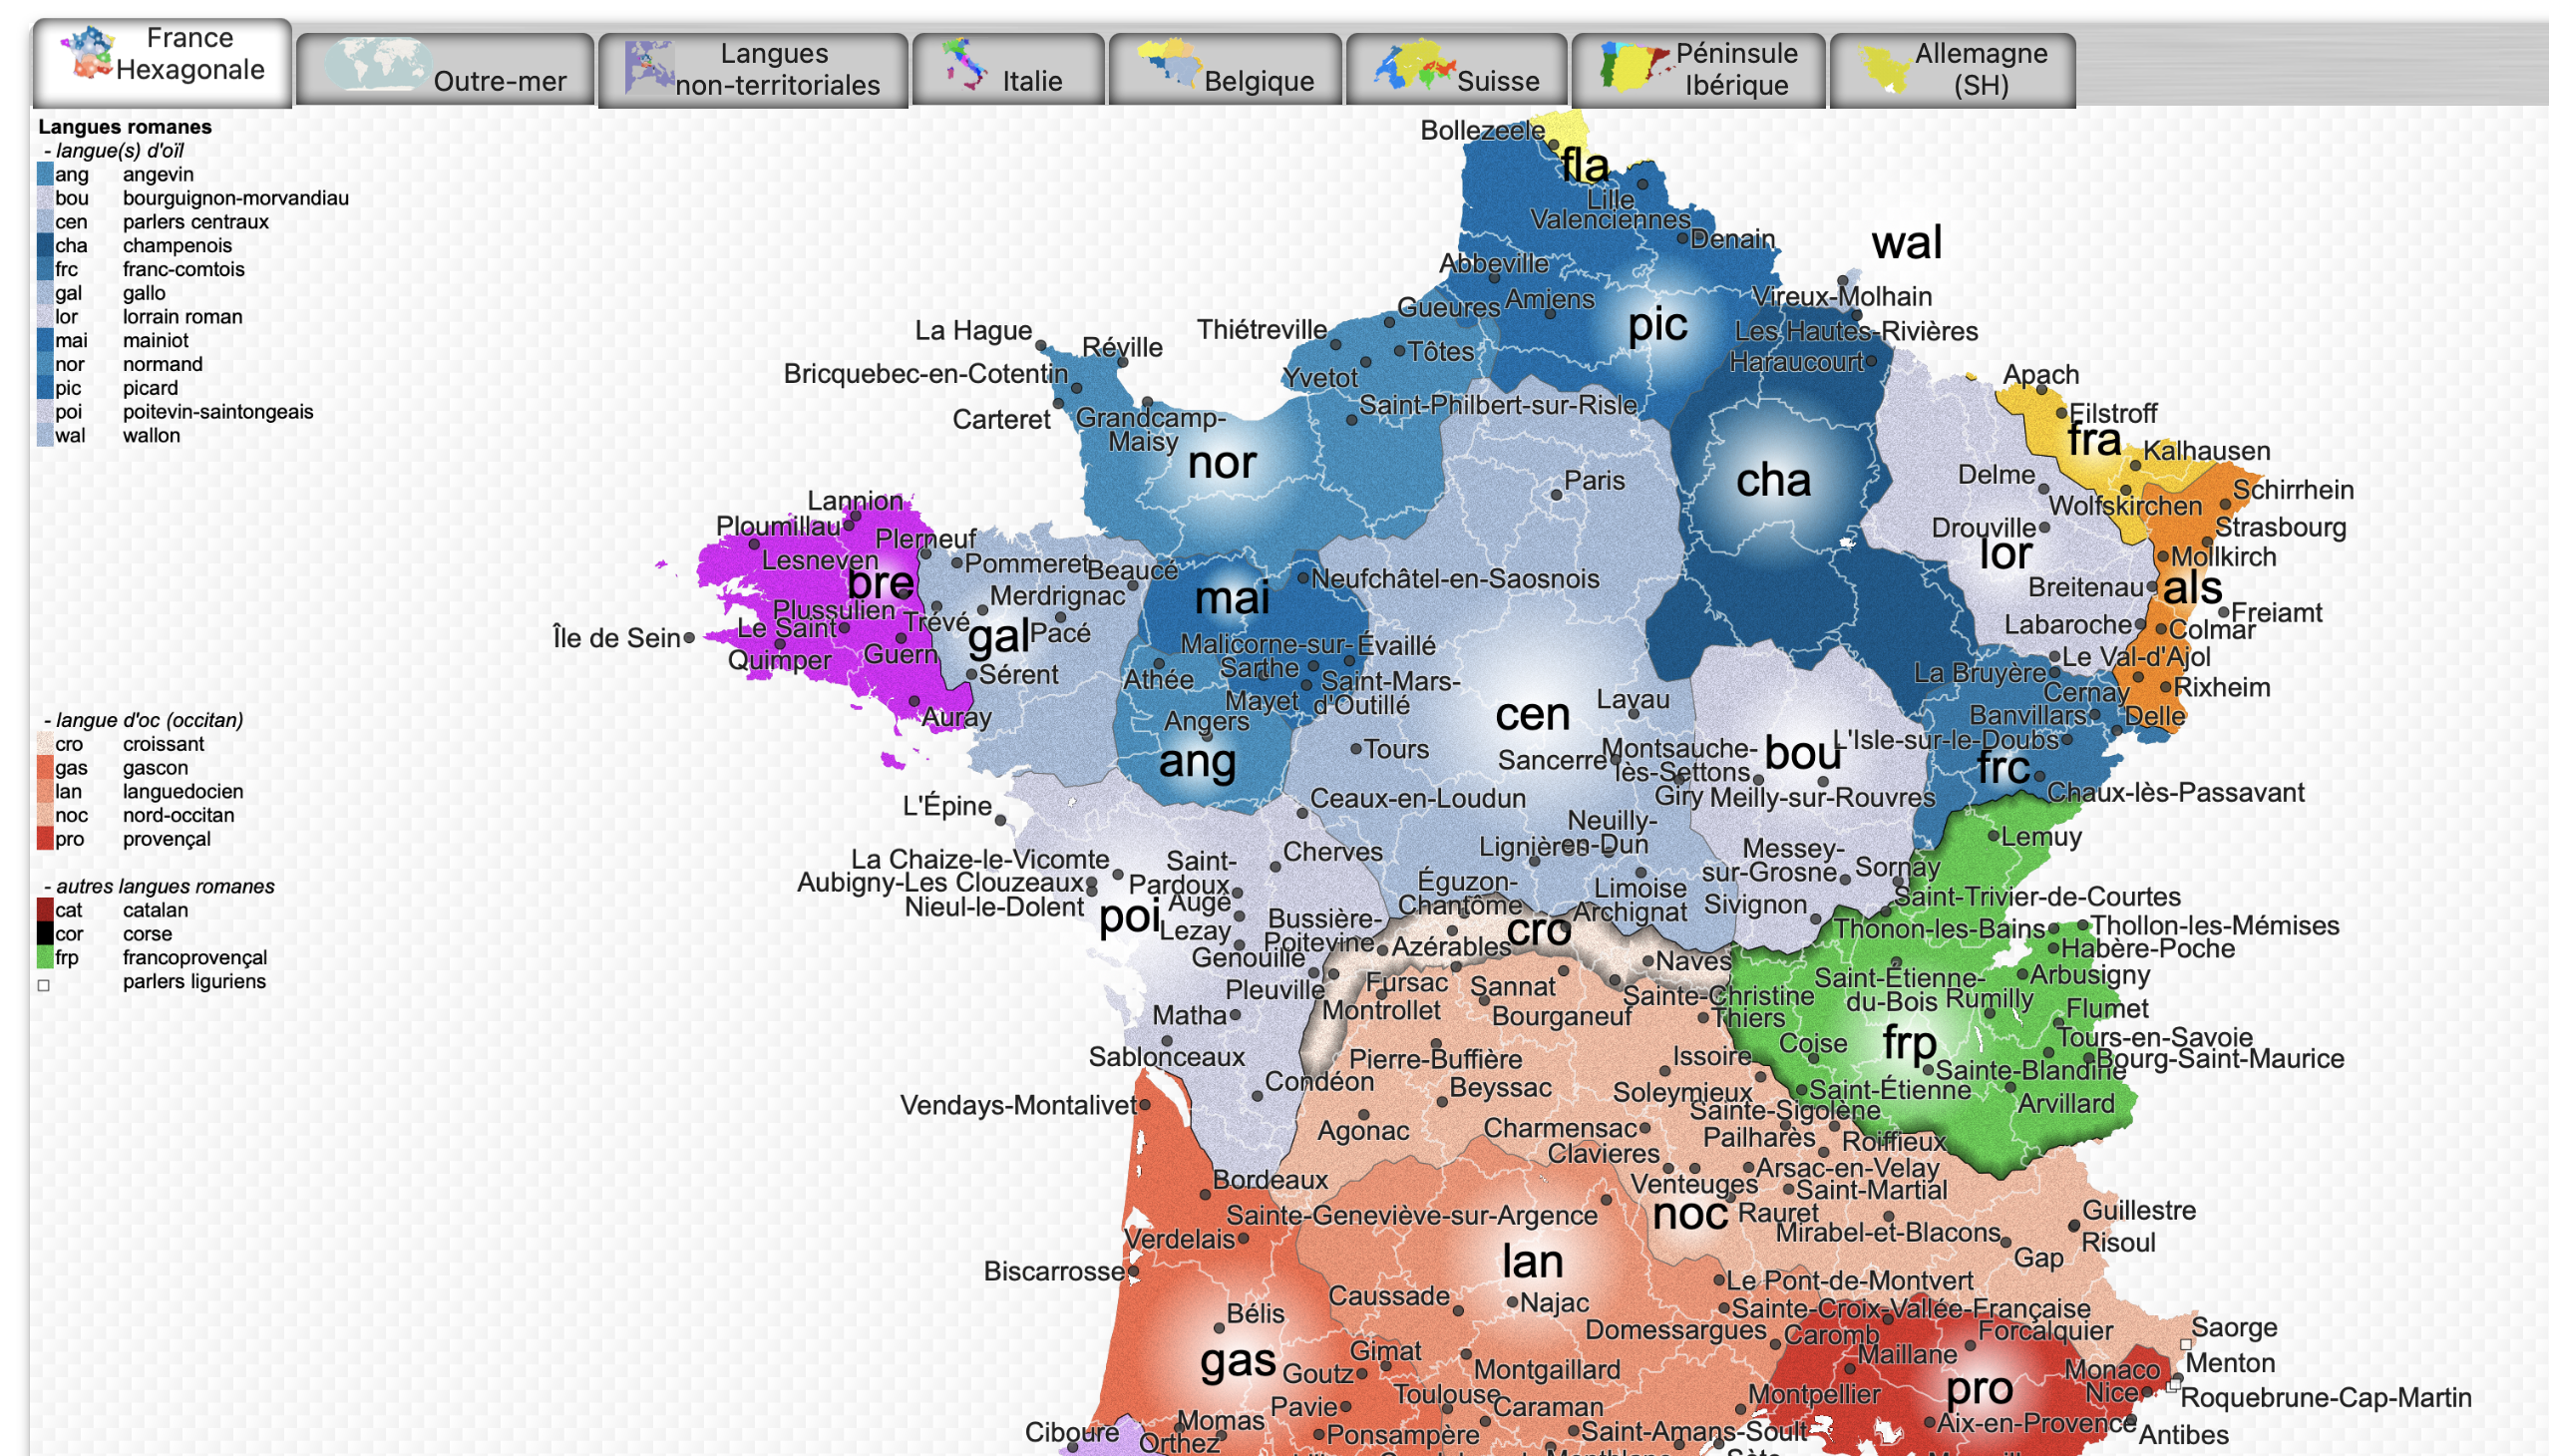
\includegraphics[width = 0.6\textwidth]{atlas}}
	\end{center}

\end{frame}


% ====================

\begin{frame}{Bases de données}{Corpus de français parlé au Québec}

	\begin{itemize}
		\item \mylink{https://applis.flsh.usherbrooke.ca/cfpq/}{applis.flsh.usherbrooke.ca/cfpq/}
	\end{itemize}

	\begin{center}
		\fbox{\includegraphics[width = 0.6\textwidth]{QF}}
	\end{center}

\end{frame}



% =====================

% =====================



% ==================

% ==================


\begin{transitionframe}


	Intro à R


\end{transitionframe}

% ====================



% ==================

\begin{frame}{Questionnaire}{\mylink{https://forms.office.com/r/XgXnS2Y8wD}{forms.office.com/r/XgXnS2Y8wD}}

	\begin{center}
		\includegraphics[width = 0.4\textwidth]{qr.png}
	\end{center}

	% Some questions related to the reading material (1--7 Barnier 2023); intro to R etc.

\end{frame}

% ====================


% \begin{frame}{Pratique}
%
% 	\begin{enumerate}
% 		\item Créer un \lav{projet R} pour notre cours
% 		\item Organiser nos dossiers : \fbox{consultez le tutoriel \mylink{https://fr.gdgarcia.ca/lng-1100/0-fichiers}{ici}}
% 		\item Créer notre premier script pour aujourd'hui
% 	\end{enumerate}
%
% \end{frame}


% ====================

% \begin{frame}{Projet R pour LNG-1100}
%
% 	\begin{enumerate}
% 		\item File $>$ New Project...
% 		\item[] Choisissez l'option 1 si vous n'avez pas encore un dossier pour le cours
% 	\end{enumerate}
%
% 	\begin{center}
% 		\fbox{\includegraphics[width = 0.4\textwidth]{project.png}}
% 		\fbox{\includegraphics[width = 0.4\textwidth]{project2.png}}
% 	\end{center}
%
% \end{frame}

% ====================


\begin{frame}{Projet R pour LNG-1100}{Pourquoi un projet...?}


	\begin{itemize}
		\item On concentre tous les fichiers du cours dans un seul dossier (dépôt Git)
		\item RStudio connaîtra déjà la localisation des fichiers à partir du fichier \var{project.Rproj}
		\item[]
		\item[] Maintenant, on continue sur RStudio
		\item[\winner] Voici la structure de notre dépôt Git :
	\end{itemize}


	\begin{center}
		\begin{tikzpicture}[scale = 0.8, level distance = 30pt]
			\tikzset{edge from parent/.style=
					{draw, edge from parent path={(\tikzparentnode.south)
								-- +(0,-8pt) -| (\tikzchildnode)}}}
			\Tree[.{\faGithub { LNG1100}}
					[.{{\faFolder} diapos} ]
					[.{{\faFolder} donnees} ]
					[.{{\faFolder} scripts} ]
					[.{{\faFolder} solutions} ]
					[.{project.Rproj} ]
					[.README.md ]
			]
		\end{tikzpicture}
	\end{center}

\end{frame}

% ============


% \begin{frame}{Nos fichiers aujourd'hui}
%
% 	\begin{center}
% 		\begin{tikzpicture}[scale = 0.72, rotate = 0]
% 			\tikzset{edge from parent/.style=
% 					{draw, thick,
% 						edge from parent fork right},every tree node/.style={align=right, anchor = base west},grow'=right}
% 			\tikzset{level distance=130pt}
% 			\tikzset{level 3/.style={sibling distance = 20pt}}
% 			\Tree[.{\faFolderOpen { LNG-1100}}
% 					[.LNG-1100.RProject ]
% 					[.{{\faFolderOpen} Donnees}
% 							[.{{\faFileO} \var{feedbackData.csv}} ]
% 							[.{{\faFileO} \var{rClauseData.csv}} ]
% 							[.{{\faFileO} \var{sampleData.csv}} ]
% 					]
% 					[.{{\faFolderOpen} Seances}
% 							[.{{\faFolderOpen} LNG-1100-2}
% 									[.{{\faFileO} \var{script_1.R}} ]
% 									[.{{\faFileO} \var{script_2.R}} ]
% 							]
% 							[.{{\faFolderOpen} LNG-1100-3} ]
% 							[.{{\faFolderOpen} ...} ]
% 					]
% 			]
%
% 		\end{tikzpicture}
% 	\end{center}
%
%
% \end{frame}


% ===============

% \begin{frame}{IMPORTANT}
%
% 	\begin{itemize}
% 		\item Vous pouvez décider de ne pas suivre la suggestion d'organisation que je vous donne
% 		\item[] \emph{Vous êtes libres de choisir votre propre organisation (ce n'est pas un cours d'informatique)}
% 		\item \lav{Dans ce cas-là :}
% 		      \begin{itemize}
% 			      \item je comprends que \textbf{vous savez comment naviguer dans vos dossiers et vos fichiers}
% 			      \item[\winner] je ne veux pas entendre la question \fr{C'est où le fichier?!} pendant le semestre
% 		      \end{itemize}
% 		\item[]
% 		\item[\winner] Si vous n'êtes pas capables de trouver vos fichiers, on sera bloqués
% 	\end{itemize}
%
% \end{frame}

% ===============

% ===============

% =============================
\begin{frame}\frametitle{}
	\begin{center}
		\vfill
		{\LARGE \textsc{RStudio}}
		\vfill
	\end{center}\end{frame}
% =============================

% \begin{frame}[fragile]{Synthèse : Les commandes et les fonctions d'aujourd'hui}
%
% 	\begin{Verbatim}
% 		read_csv(...)                    # importer un fichier csv
% 		write_csv(...)                   # exporter un fichier csv
% 		mean(...)                        # moyenne
% 		sd(...)                          # écart-type
% 		summarize(, .by = ...)           # créer un résumé avec n nouvelles colonnes
% 		tribble(...)                     # créer un tableau (tibble) manuellement
% 		glimpse(...)                     # visualiser les colonnes comme lignes
% 		# (idéal pour les tableaux avec plusieurs colonnes)
% 		pivot_longer(names_to = "...",   # transformation « wide-to-long »
% 		values_to = "...",
% 		col = ...:...)
% 		mutate(...)
% 		filter(...)
% 		select(...)
%
% 		# Le « pipe » (|>) combine les fonctions d'une façon intuitive
% 		donnees |>
% 		mutate(...) |>               # créer des colonnes
% 		filter(...) |>               # filtrer les données
% 		select(...) |>               # sélectionner quelques colonnes
% 		summarize(...)               # créer un résumé
% 	\end{Verbatim}
%
% \end{frame}

% =================

\appendix
\begin{frame}[allowframebreaks]

	{
		\footnotesize
		\frametitle{Références}
		\bibliographystyle{apalike}
		\bibliography{../../../../Dropbox/Academia/References/references}
	}

\end{frame}



%%%%%%%%%%%%%%%%%%%%%%%%%% APPENDIX

%%%%%%%%%%%%%%%%%%%%%%%%%%%%%%%%%%%%%%%%%%%%%%%%


%\begin{frame}{Annexe i}
%
%\begin{center}
%	...
%\end{center}
%  
%\end{frame}


\end{document}
